\chapter{Laboratório e Experimento XYZ, por <Estudante> (<githubusername>)\label{desenho:experimento:jhcf}}

\section{Introdução}

Este capítulo apresenta a construção e uso do laboratório de simulações <xyz> para a realização de experimentos que tem por objetivo investigar a hipótese causal <nomear a hipótese causal> que relaciona variáveis independentes e variáveis dependentes, supostamente presente nos estudos bibliométricos por mim realizados e disponíveis em \ref{chap:bibliometria:jhcf}.

É composto por mais cinco seções: 
\begin{enumerate}
    \item Descrição do fenômeno real;
    \item Apresentação do laboratório de simulações;
    \item Apresentação de análises exploratórias dos dados de experimentos realizados com o uso do laboratório;
    \item Discussão sobre \textit{insights} obtidos após os experimentos; e
    \item Conclusões.
\end{enumerate}

\section{O Fenômeno do Mundo Real}

Descrever o fenômeno do mundo real que está sendo modelado pelo laboratório, seja ele social, biológico, ecológico, físico, químico etc.

Complementar com figuras, imagens ou descrições exemplificando o fenômeno real.

Nas descrições do fenômeno, usar o suporte de pelo menos duas referências bibliográficas, obtidas com a sua pesquisa bibliométrica.
Inserir ou usar a referência no repositório RESIC e usar o mecanismo de citações no \LaTeX.

coloque as referências usadas na coleção 
\begin{verbatim}
    _Disciplinas/ComputExperimental/20221/<githubusername>
\end{verbatim}
Exporte toda a biblioteca RESIC e atualize o arquivo RESIC.bib, para poder citar as referências que você incluiu na biblioteca, por exemplo \cite{gregoire_professional_2021}

\section{O Laboratório <XYZ>}

Iniciar a seção com uma descrição, de forma breve, do que trata o laboratório <XYZ>, porque ele é interessante etc.

\subsection{O Conceito da Simulação}

Apresentar e citar (com referências) a partir de onde o código da simulação foi obtido.

Apresentar suposições na arquitetura multiagente do simulador, para simular o fenômeno no mundo real.

Apresentar o contexto da simulação e os fenômenos de interesse explorados no laboratório, de forma textual.

\subsection{O Simulador}

Apresentar o simulador, suas principais variáveis (independentes, dependentes e de controle) presentes no código e na interface da simulação.
Apresentar a interface com o usuário da simulação de forma textual e gráfica.

\subsubsection{Variáveis Independentes ou de Controle}

São as seguintes as variáveis Independentes ou de Controle, manipuláveis na interface gráfica do simulador:
\begin{description}
\item [X] <Descrever>
\item [Y] <Descrever>
\item [Z] <Descrever>
\end{description}

\subsubsection{Variáveis Dependentes}

São as seguintes as variáveis Dependentes, cujos valores são coletados e apresentados na interface gráfica do simulador:
\begin{description}
\item [X] <Descrever>
\item [Y] <Descrever>
\item [Z] <Descrever>
\end{description}

Recomenda-se que pelo menos uma das variáveis dependentes deve representar uma condição coletiva do modelo, isso é, não pode ser uma simples contagem de uma variável de estado do agente.

\subsection{A Hipótese Causal}

Motivar e apresentar a hipótese causal de forma textual.

Apresentar e citar pelo menos duas referências bibliográficas que suportam a sua hipótese causal.

%Apresentar a hipótese causal modelada com o uso da ferramenta Loopy.

%Apresentar, de forma gráfica, exemplos de execução da hipótese causal, na ferramenta Loopy.

% \begin{figure}
%     \centering
%     \includegraphics[width=0.5\textwidth]{experiments/jhcf/ExperimentoProducaoCiencia/Causal.png}
%     \caption{Modelo causal de simulação XYZ. Para ver o modelo visite  \url{https://bit.ly/3qDmXwj}.}
%     \label{fig:jhcf:EXP:xyz:modelo:causal}
% \end{figure}

% \begin{figure}
%     \centering
%     \includegraphics[width=0.5\textwidth]{experiments/jhcf/ExperimentoProducaoCiencia/Simulacao.png}
%     \caption{Simulação do modelo causal de simulação XYZ. }
%     \label{fig:jhcf:EXP:xyz:simulacao:modelo:causal}
% \end{figure}

% Prover uma url (usar o bit.ly, conforme indica a interface gráfica do Loopy, na opção ``Save as link'') para que o leitor possa ele mesmo executar a simulação no Loopy.

\subsection{O Código do Simulador}

Justificar o alinhamento entre o código do simulador e a hipótese causal.

Apresentar todas as classes que fazem parte do código do simulador.

Apresentar, usando o pacote lstlistings, os principais trechos e linhas de código do simulador, especialmente os seguintes:
\begin{description}
\item [Criação do modelo e agentes]
\item [Comportamento do modelo e dos agentes a cada passo]
% \item [Simulador batch].
\end{description}

% \lstinputlisting[numbers=left,language={Python},basicstyle=\tiny\ttfamily,caption={Código da Criação de um agente.},label={code:jhcf:EXP:xyz:batch:run},firstnumber=110,firstline=110,lastline=127]
% {labs/jhcf/ExperimentoProducaoCiencia/model.py}


%Observe que a descrição do simulador batch deve ser suficientemente detalhada para evidenciar o desenho do experimento, a seleção e (ou) coleta de valores das variáveis independentes, de controle e dependentes.

\section{Os Experimentos Realizados}

Dizer quando e quantos foram os experimentos realizados, e com qual  objetivo. Fazer os experimentos apenas de forma interativa, usando o simulador, em várias execuções, para ganhar intuição sobre a dinâmica ou comportamento do fenômeno, buscando identificar relações de causa e efeito entre as variáveis independentes e dependentes.

Apresentar problemas e dificuldades com execução dos experimentos (apenas simulações), se foram superados ou não.

Mostrar graficamente pelo menos um exemplo de simulação.

\begin{figure}
    \centering
    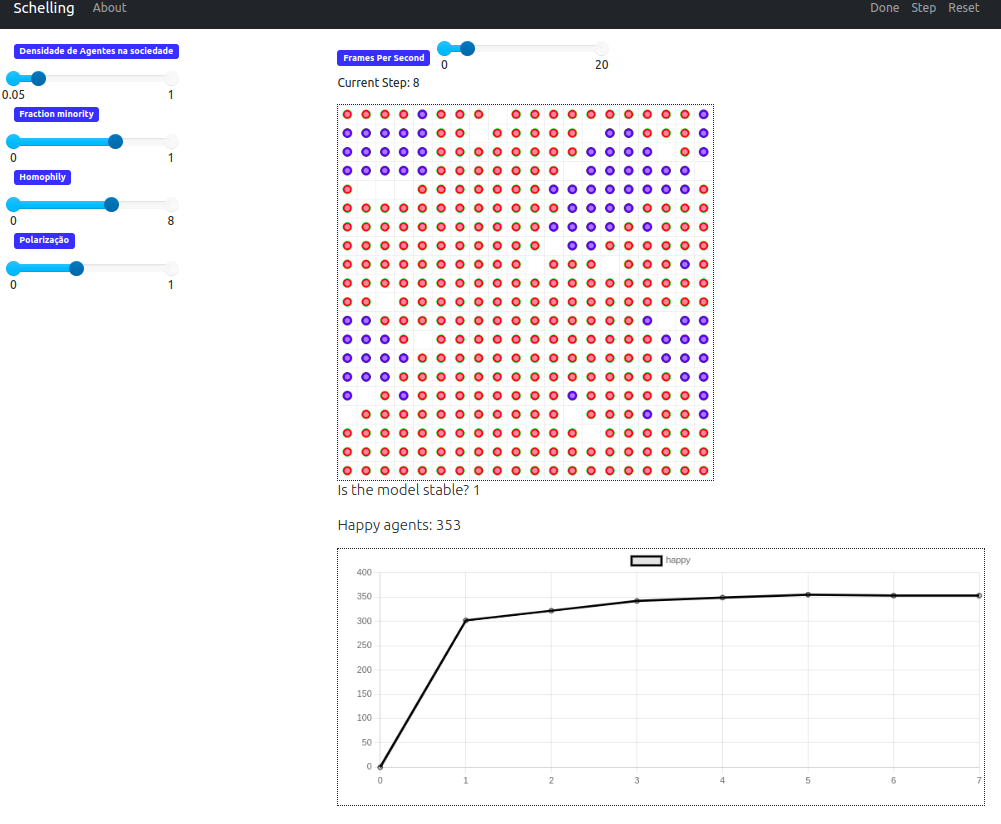
\includegraphics[width=0.9\textwidth]{3-Simulando-Um-Fenomeno/tarefas/T6-Aprimoramento-Simulacao/estudantes/tarefa-jhcf/simul-polariz-0.1-20221216.png}
    \caption{Interface gráfica do simulador polarizacão.}
    \label{fig:jhcf:polariza}
\end{figure}

A figura \ref{fig:jhcf:polariza} apresenta a interface gráifca para o simulador, onde se destacam 4 painéis: superior, esquerda, centro superior, cesntro inferior.

A simulação usando um valor baixo para a polarização converge para um estado estável em oito passos.

%Um projeto de \gls{SI} pode ser validado com simulações.
% \subsection{Os Dados Coletados}

% Apresentar e descrever cada um dois tipos de dados coletados, e as variáveis presentes em cada CSV.

% Variáveis no arquivo do modelo:
% \begin{description}
% \item [X] <Descrever>
% \item [Y] <Descrever>
% \item [Z] <Descrever>
% \end{description}

% Variáveis no arquivo dos agentes:
% \begin{description}
% \item [X] <Descrever>
% \item [Y] <Descrever>
% \item [Z] <Descrever>
% \end{description}

% Exemplificar alguns registros presentes em cada um dos arquivos, usando o comando csvreader. 
% Ver exemplo a seguir.


% \begin{table}[htp]
%     \centering
% \footnotesize
% \csvreader[
% separator=comma, % especifica o separador de colunas
% tabular = {|r|l|r|r|r|r|}, 
% filter={\value{csvrow}<20}, % indica quantas colunas devem ser apresentadas
% %,filter not strcmp={\csvcolii}{},
% table head = \hline\hline \# & Initial Trading \%	& Alpha & Beta & Available & Decease Rate\\ \hline\hline, % cabeçalho da tabela
% table foot = \hline\hline] % rodapé da tabela
% {experiments/jhcf/ExperimentoProducaoCiencia/data.csv} % arquivo de onde os dados devem ser lidos
% {InitialTradingPerc=\trading,AlphaAjuste=\salpha,BetaAjuste=\sbeta,Available=\avail,ChannelsDeceasedRate=\deceaserate} % mapeia os nomes das colunas no CSV para variáveis a serem usadas na linha de detalhe, abaixo
% { \thecsvrow & \trading & \salpha & \sbeta & \avail & \deceaserate} % valores a serem mostrados nas linhas
% \caption{Apresentando alguns  registros mantidos em um arquivo CSV.}
%     \label{tab:jhcf:EXP:xyz:registros:modelo}
% \end{table}

% \subsection{Análises exploratórias preliminares}

% Apresentar as distribuições de frequência dos valores obtidos para as variáveis dependentes, em função de cada configuração de valores para variáveis independentes.

% Plotar graficamente essas distribuições de frequência e discutir as variações observadas, em termos de média (ou moda) e desvio padrão. Constatar a normalidade ou não normalidade das distribuições de frequência, quando possível.

% Nas plotagens, usar o R Studio, com o comando hist(). Ao gerar as plotagens no R Studio, usar a opção ``Plots -> Export -> Save as PDF'', para que as imagens sejam geradas de forma vetorial, e não percam qualidade quando redimensionadas.


% \begin{figure}
%     \centering
%     \includegraphics[page=1,clip=true,trim={0 1cm 1.5cm 2cm},width=\textwidth,height=0.5\textheight]{experiments/jhcf/ExperimentoProducaoCiencia/Rplot02.pdf}
%     \caption{Distribuição de Frequência no número de nós infectados em 300 experimentos, após 100 passos de simulação em cada experimento, com numNodes==100, virusSpreadChance==0.9.}
%     \label{fig:jhcf:EXP:xyz:distfreq}
% \end{figure}


\section{Discussão e \textit{insights} preliminares sobre as hipóteses}

Argumentar textualmente, com base nas características reais do fenômeno modelado, na hipótese causal, nos fundamentos do desenho do simulador, e nos experimentos (simulações) interativos, se a hipótese causal inicial parece ter sido comprovada ou refutada \textbf{pelas observações da execução das simulações}.

\section{Conclusão}

Relatar as aprendizagens e dúvidas sobre a experiência do exercício.
